\documentclass[12pt]{../../vespers-sheet} %booklet
\usepackage{multicol}

\begin{document}

% TODO: Update the title for the specific feast
\chapter*{Terce of Our Lady of the Holy Rosary}

\begin{center}
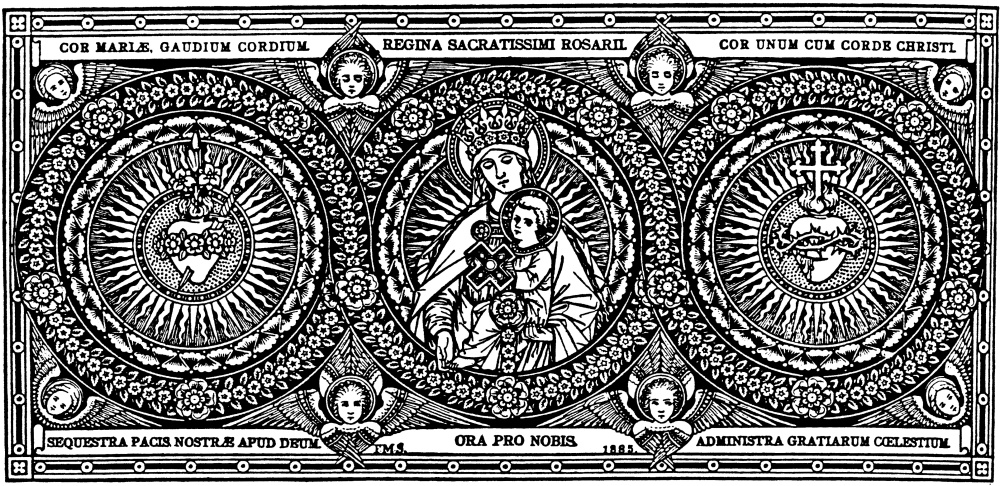
\includegraphics[width=\textwidth]{lady-of-the-rosary}
\end{center}

\vfill\pagebreak

%\section*{Beginning of the Office}

\begin{rubricbox}

{\color{red} All make the sign of the cross with the Officiant as he intones:}

\end{rubricbox}

% TODO: Make sure that the tone of the deus adjutorium matches the season primarily and the solemnity of the feast secondarily
 \gresetinitiallines{1}
\gregorioscore{../../common/deus-in-adjutorium-ferial}

\textit{
O God, come to my assistance.
{\color{red}\Vbar.}~O Lord, make haste to help me.
Glory be to the Father, and to the Son, and to the Holy Spirit,
as it was in the beginning, is now, and ever shall be, world without end. Amen.
Praise to Thee, O Lord, King of endless glory.}

\section*{Hymn}

\textit{\color{red}The Cantor leads the hymn:}

\gresetinitiallines{1}
\gregorioscore{../../hymns/nunc_sancte_nobis_BMV}

{\itshape
	1.  Come Holy Ghost who ever One
	Art with the Father and the Son,
	It is the hour, our souls possess
	With thy full flood of holiness.
	
	2. Let flesh and heart and lips and mind
	Sound forth our witness to mankind;
	And love light up our mortal frame,
	Till others catch the living flame.
	
	3. All honour, laud, and glory be,
	O Jesu, Virgin-Born, to thee;
	Whom with the Father we adore,
	And Holy Ghost, for evermore.
	Amen.
}

%%

\section*{Psalm 118:33-48}

\textit{\textnormal{Ant. 1.} God is gone up with a shout,
\textnormal{Ps.} Set before me for a law the way of thy justifications, O Lord:}

\gresetinitiallines{1}
\gregorioscore{ps118-antiphon}

\gresetinitiallines{0}
\gregorioscore{ps118-intonation}

\begin{latinenglishsection}

\latinenglish{

	2. Da mihi intelléctum, et scrutábor \textit{le}\textit{gem} \textbf{tu}am:~* et custódiam illam in to\textit{to} \textit{cor}\textit{de} \textbf{me}o.

3. Deduc me in sémitam mandató\textit{rum} \textit{tu}\textbf{ó}rum:~* qui\textit{a} \textit{ip}\textit{sam} \textbf{vó}lui.

4. Inclína cor meum in testimó\textit{ni}\textit{a} \textbf{tu}a:~* et non \textit{in} \textit{a}\textit{va}\textbf{rí}tiam.

5. Avérte óculos meos ne vídeant \textit{va}\textit{ni}\textbf{tá}tem:~* in via tua \textit{vi}\textit{ví}\textit{fi}\textbf{ca} me.

6. Státue servo tuo eló\textit{qui}\textit{um} \textbf{tu}um,~* in \textit{ti}\textit{mó}\textit{re} \textbf{tu}o.

7. Amputa oppróbrium meum quod \textit{su}\textit{spi}\textbf{cá}tus sum:~* quia judícia \textit{tu}\textit{a} \textit{ju}\textbf{cún}da.

8 .Ecce concupívi man\textit{dá}\textit{ta} \textbf{tu}a:~* in æquitáte tua \textit{vi}\textit{ví}\textit{fi}\textbf{ca} me.

9. Et véniat super me misericórdia \textit{tu}\textit{a}, \textbf{Dó}mine:~* salutáre tuum secúndum e\textit{ló}\textit{qui}\textit{um} \textbf{tu}um.

10. Et respondébo exprobrántibus \textit{mi}\textit{hi} \textbf{ver}bum:~* quia sperávi in ser\textit{mó}\textit{ni}\textit{bus} \textbf{tu}is.

11. Et ne áuferas de ore meo verbum veritátis \textit{us}\textit{que}\textbf{quá}que:~* quia in judíciis tuis \textit{su}\textit{per}\textit{spe}\textbf{rá}vi.

12. Et custódiam legem \textit{tu}\textit{am} \textbf{sem}per:~* in s\'{\ae}culum et in \textit{s\'{\ae}}\textit{cu}\textit{lum} \textbf{s\'{\ae}}culi.

13. Et ambulábam in \textit{la}\textit{ti}\textbf{tú}dine:~* quia mandáta tu\textit{a} \textit{ex}\textit{qui}\textbf{sí}vi.

14. Et loquébar in testimóniis tuis in con\textit{spéc}\textit{tu} \textbf{re}gum:~* et \textit{non} \textit{con}\textit{fun}\textbf{dé}bar.

15. Et meditábar in man\textit{dá}\textit{tis} \textbf{tu}is,~* \textit{quæ} \textit{di}\textbf{lé}xi.

16. Et levávi manus meas ad mandáta tua, \textit{quæ} \textit{di}\textbf{lé}xi:~* et exercébar in justificati\textit{ó}\textit{ni}\textit{bus} \textbf{tu}is.

{\color{red}\textit{(bow)}} Glória Pa\textit{tri}, \textit{et} \textbf{Fí}lio,~* et Spi\textit{rí}\textit{tu}\textit{i} \textbf{Sanc}to.

{\color{red}\textit{(rise)}} Sicut erat in princípio, et \textit{nunc}, \textit{et} \textbf{sem}per,~* et in s\'{\ae}cula sæ\textit{cu}\textit{ló}\textit{rum}. \textbf{A}men. %% 

}{
	2. Give me understanding, and I will search thy law; * and I will keep it with my whole heart.

3. Lead me into the path of thy commandments; * for this same I have desired.

4. Incline my heart into thy testimonies * and not to covetousness.

5. Turn away my eyes that they may not behold vanity: * quicken me in thy way.

6. Establish thy word to thy servant, * in thy fear.

7. Turn away my reproach, which I have apprehended: * for thy judgments are delightful.

8. Behold I have longed after thy precepts: * quicken me in thy justice.

9. Let thy mercy also come upon me, O Lord: * thy salvation according to thy word.

10. So shall I answer them that reproach me in any thing; * that I have trusted in thy words.

11. And take not thou the word of truth utterly out of my mouth: * for in thy words, I have hoped exceedingly.

12. So shall I always keep thy law, * for ever and ever.

13. And I walked at large: * because I have sought after thy commandments.

14. And I spoke of thy testimonies before kings: * and I was not ashamed.

15. I meditated also on thy commandments, * which I loved.

16. And I lifted up my hands to thy commandments, which I loved: * and I was exercised in thy justifications.

17. Glory be to the Father, and to the Son, * and to the Holy Ghost.

18. As it was in the beginning, is now, * and ever shall be, world without end. Amen. %%
}

\end{latinenglishsection}

%%

\section*{Psalm 118:49-64}

\begin{latinenglishsection}

\latinenglish{

	2. Hæc me consoláta est in humili\textit{tá}\textit{te} \textbf{me}a:~* quia elóquium tuum \textit{vi}\textit{vi}\textit{fi}\textbf{cá}vit me.

3. Supérbi iníque agébant \textit{us}\textit{que}\textbf{quá}que:~* a lege autem tua \textit{non} \textit{de}\textit{cli}\textbf{ná}vi.

4. Memor fui judiciórum tuórum a s\'{\ae}\textit{cu}\textit{lo}, \textbf{Dó}mine:~* \textit{et} \textit{con}\textit{so}\textbf{lá}tus sum.

5. Deféctio \textit{té}\textit{nu}\textbf{it} me,~* pro peccatóribus derelinquénti\textit{bus} \textit{le}\textit{gem} \textbf{tu}am.

6. Cantábiles mihi erant justificati\textit{ó}\textit{nes} \textbf{tu}æ,~* in loco peregrina\textit{ti}\textit{ó}\textit{nis} \textbf{me}æ.

7. Memor fui nocte nóminis \textit{tu}\textit{i}, \textbf{Dó}mine:~* et custodí\textit{vi} \textit{le}\textit{gem} \textbf{tu}am.

8. Hæc fac\textit{ta} \textit{est} \textbf{mi}hi:~* quia justificatiónes tu\textit{as} \textit{ex}\textit{qui}\textbf{sí}vi.

9. Pórtio \textit{me}\textit{a}, \textbf{Dó}mine,~* dixi custodí\textit{re} \textit{le}\textit{gem} \textbf{tu}am.

10. Deprecátus sum fáciem tuam in toto \textit{cor}\textit{de} \textbf{me}o:~* miserére mei secúndum e\textit{ló}\textit{qui}\textit{um} \textbf{tu}um.

11. Cogitávi \textit{vi}\textit{as} \textbf{me}as:~* et convérti pedes meos in testi\textit{mó}\textit{ni}\textit{a} \textbf{tu}a.

12. Parátus sum, et non \textit{sum} \textit{tur}\textbf{bá}tus:~* ut custódiam \textit{man}\textit{dá}\textit{ta} \textbf{tu}a.

13. Funes peccatórum circum\textit{plé}\textit{xi} \textbf{sunt} me:~* et legem tuam \textit{non} \textit{sum} \textit{ob}\textbf{lí}tus.

14. Média nocte surgébam ad confi\textit{tén}\textit{dum} \textbf{ti}bi:~* super judícia justifica\textit{ti}\textit{ó}\textit{nis} \textbf{tu}æ.

15. Párticeps ego sum ómnium ti\textit{mén}\textit{ti}\textbf{um} te:~* et custodiéntium \textit{man}\textit{dá}\textit{ta} \textbf{tu}a.

16. Misericórdia tua, Dómine, ple\textit{na} \textit{est} \textbf{ter}ra:~* justificatió\textit{nes} \textit{tu}\textit{as} \textbf{do}ce me.

{\color{red}\textit{(bow)}} Glória Pa\textit{tri}, \textit{et} \textbf{Fí}lio,~* et Spi\textit{rí}\textit{tu}\textit{i} \textbf{Sanc}to.

{\color{red}\textit{(rise)}} Sicut erat in princípio, et \textit{nunc}, \textit{et} \textbf{sem}per,~* et in s\'{\ae}cula sæ\textit{cu}\textit{ló}\textit{rum}. \textbf{A}men. %% 

}{
	1. Be thou mindful of thy word to thy servant, * in which thou hast given me hope.

2. This hath comforted me in my humiliation: * because thy word hath enlivened me.

3. The proud did iniquitously altogether: * but I declined not from thy law.

4. I remembered, O Lord, thy judgments of old: * and I was comforted.

5. A fainting hath taken hold of me, * because of the wicked that forsake thy law.

6. Thy justifications were the subject of my song, * in the place of my pilgrimage.

7. In the night I have remembered thy name, O Lord: * and have kept thy law.

8. This happened to me: * because I sought after thy justifications.

9. O Lord, my portion, * I have said, I would keep thy law.

10. I entreated thy face with all my heart: * have mercy on me according to thy word.

11. I have thought on my ways: * and turned my feet unto thy testimonies.

12. I am ready, and am not troubled: * that I may keep thy commandments.

13. The cords of the wicked have encompassed me: * but I have not forgotten thy law.

14. I rose at midnight to give praise to thee; * for the judgments of thy justification.

15. I am a partaker with all them that fear thee, * and that keep thy commandments.

16.  The earth, O Lord, is full of thy mercy: * teach me thy justifications.

17. Glory be to the Father, and to the Son, * and to the Holy Ghost.

18. As it was in the beginning, is now, * and ever shall be, world without end. Amen. %%
}

\end{latinenglishsection}


%%

\section*{Psalm 118:65-80}

\begin{latinenglishsection}

\latinenglish{

	2. Bonitátem et disciplínam et scién\textit{ti}\textit{am} \textbf{do}ce me:~* quia mandá\textit{tis} \textit{tu}\textit{is} \textbf{cré}didi.

3. Priúsquam humiliárer e\textit{go} \textit{de}\textbf{lí}qui:~* proptérea elóquium tu\textit{um} \textit{cus}\textit{to}\textbf{dí}vi.

4. \textit{Bo}\textit{nus} \textbf{es} tu:~* et in bonitáte tua doce me justifica\textit{ti}\textit{ó}\textit{nes} \textbf{tu}as.

5. Multiplicáta est super me iníquitas\\ \textit{su}\textit{per}\textbf{bó}rum:~* ego autem in toto corde meo scrutábor \textit{man}\textit{dá}\textit{ta} \textbf{tu}a.

6. Coagulátum est sicut lac \textit{cor} \textit{e}\textbf{ó}rum:~* ego vero legem tu\textit{am} \textit{me}\textit{di}\textbf{tá}tus sum.

7. Bonum mihi quia hu\textit{mi}\textit{li}\textbf{ás}ti me:~* ut discam justifica\textit{ti}\textit{ó}\textit{nes} \textbf{tu}as.

8. Bonum mihi lex \textit{o}\textit{ris} \textbf{tu}i:~* super míllia au\textit{ri} \textit{et} \textit{ar}\textbf{gén}ti.

9. Manus tuæ fecérunt me, et \textit{plas}\textit{ma}\textbf{vé}runt me:~* da mihi intelléctum, et discam \textit{man}\textit{dá}\textit{ta} \textbf{tu}a.

10. Qui timent te vidébunt me et \textit{læ}\textit{ta}\textbf{bún}tur:~* quia in verba tua \textit{su}\textit{per}\textit{spe}\textbf{rá}vi.

11. Cognóvi, Dómine, quia ǽquitas judí\textit{ci}\textit{a} \textbf{tu}a:~* et in veritáte tua \textit{hu}\textit{mi}\textit{li}\textbf{ás}ti me.

12. Fiat misericórdia tua ut \textit{con}\textit{so}\textbf{lé}tur me:~* secúndum elóquium tu\textit{um} \textit{ser}\textit{vo} \textbf{tu}o.

13. Véniant mihi miseratiónes tu\textit{æ}, \textit{et} \textbf{vi}vam:~* quia lex tua medi\textit{tá}\textit{ti}\textit{o} \textbf{me}a est.

14. Confundántur supérbi, quia injúste iniquitátem fe\textit{cé}\textit{runt} \textbf{in} me:~* ego autem exercébor in \textit{man}\textit{dá}\textit{tis} \textbf{tu}is.

15. Convertántur mi\textit{hi} \textit{ti}\textbf{mén}tes te:~* et qui novérunt testi\textit{mó}\textit{ni}\textit{a} \textbf{tu}a.

16. Fiat cor meum immaculátum in\\ justificatió\textit{ni}\textit{bus} \textbf{tu}is,~* \textit{ut} \textit{non} \textit{con}\textbf{fún}dar.

{\color{red}\textit{(bow)}} Glória Pa\textit{tri}, \textit{et} \textbf{Fí}lio,~* et Spi\textit{rí}\textit{tu}\textit{i} \textbf{Sanc}to.

{\color{red}\textit{(rise)}} Sicut erat in princípio, et \textit{nunc}, \textit{et} \textbf{sem}per,~* et in sǽcula sæ\textit{cu}\textit{ló}\textit{rum}. \textbf{A}men. %% 

}{
	1. Thou hast done well with thy servant, O Lord, * according to thy word.

2. Teach me goodness and discipline and knowledge; * for I have believed thy commandments.

3. Before I was humbled I offended; * therefore have I kept thy word.

4. Thou art good; * and in thy goodness teach me thy justifications.

5. The iniquity of the proud hath been multiplied over me: * but I will seek thy commandments with my whole heart.

6. Their heart is curdled like milk: * but I have meditated on thy law.

7. It is good for me that thou hast humbled me, * that I may learn thy justifications.

8. The law of thy mouth is good to me, * above thousands of gold and silver.

9. Thy hands have made me and formed me: * give me understanding, and I will learn thy commandments.

10. They that fear thee shall see me, and shall be glad: * because I have greatly hoped in thy words.

11. I know, O Lord, that thy judgments are equity: * and in thy truth thou hast humbled me.

12. O! let thy mercy be for my comfort, * according to thy word unto thy servant.

13. Let thy tender mercies come unto me, and I shall live: * for thy law is my meditation.

14. Let the proud be ashamed, because they have done unjustly towards me: * but I will be employed in thy commandments.

15. Let them that fear thee turn to me: * and they that know thy testimonies.

16. Let my heart be undefiled in thy justifications, * that I may not be confounded.

17. Glory be to the Father, and to the Son, * and to the Holy Ghost.

18. As it was in the beginning, is now, * and ever shall be, world without end. Amen. %%
}

\end{latinenglishsection}

\gresetinitiallines{1}
\gregorioscore{ps118-antiphon}

%%

\vfill\pagebreak

\section*{Chapter Responsory Verse}

\textit{\color{red}The Officiant leads the Chapter and responsory:}

\begin{latinenglishsection}

\latinenglish{
	In me grátia omnis viæ et veritátis, in me omnis spes vi\textbf{tæ} \textit{et vir}\textbf{tú}tis. Ego, quasi rosa plantáta super rivos aquárum, fructificávi.
}{
	In me is all grace of the way and of the truth; in me is all hope of life and virtue; I have flowered forth like a rose planted by the brooks of water.
}

\end{latinenglishsection}

\gresetinitiallines{1}
\gregorioscore{chapter_responsory}

\gresetinitiallines{0}
\gabcsnippet{(c3) <c><sp>V/</sp>.</c> Post(h) par(h)tum(h) Vir(h)go(h) in(h)vi(h)o(h)lá(h)ta(h) per(h)man(h)sís(h)ti(f). (::)}

\gresetinitiallines{0}
\gabcsnippet{(c3) <c><sp>R/</sp>.</c> De(h)i(h) Gé(h)ni(h)trix(h) in(h)ter(h)cé(h)de(h) pro(h) no(h)bis(f). (::)}


%\begin{latinenglishsection}

%\latinenglish{
%	In me grátia omnis viæ et veritátis, in me omnis spes vi\textbf{tæ} \textit{et vir}\textbf{tú}tis. Ego, quasi rosa plantáta super rivos aquárum, fructificávi.
%	
%	{\color{red}\Rbar.}~Deo grátias.
%	
%	{\color{red}\Rbar.br} Sancta Dei Génitrix, * Semper Virgo María.
%	{\color{red}\Rbar.} Sancta Dei Génitrix, * Semper Virgo María.\\
%	{\color{red}\Vbar.} Intercéde pro nobis ad Dóminum, Deum nostrum.\\
%	{\color{red}\Rbar.} Semper Virgo María.\\
%	{\color{red}\Vbar.} Glória Patri, et Fílio, * et Spirítui Sancto.\\
%	{\color{red}\Rbar.} Sancta Dei Génitrix, * Semper Virgo María.
%	
%	{\color{red}\Vbar.} Post partum, Virgo, invioláta permansísti.
%	{\color{red}\Rbar.} Dei Génitrix, intercéde pro nobis.
%}{
%	In me is all grace of the way and of the truth; in me is all hope of life and virtue; I have flowered forth like a rose planted by the brooks of water.
%	
%	 {\color{red}\Rbar.}~Thanks be to God.
%	 
%	{\color{red}\Rbar.br} Holy Mother of God, * Mary always a Virgin.
%	{\color{red}\Rbar.} Holy Mother of God, * Mary always a Virgin.
%	{\color{red}\Vbar.} Intercede for us with the Lord our God.
%	{\color{red}\Rbar.} Mary always a Virgin.
%	{\color{red}\Vbar.} Glory be to the Father, and to the Son, * and to the Holy Ghost.
%	{\color{red}\Rbar.} Holy Mother of God, * Mary always a Virgin.
%	
%	{\color{red}\Vbar.} After childbirth thou still remainest a Virgin.
%	{\color{red}\Rbar.} Mother of God, pray for us.
%}
%
%\end{latinenglishsection}

{\itshape
	In me is all grace of the way and of the truth; in me is all hope of life and virtue; I have flowered forth like a rose planted by the brooks of water.
	
	 {\color{red}\Rbar.}~Thanks be to God.
	 
	{\color{red}\Rbar.br} Holy Mother of God, * Mary always a Virgin.
	{\color{red}\Rbar.} Holy Mother of God, * Mary always a Virgin.
	{\color{red}\Vbar.} Intercede for us with the Lord our God.
	{\color{red}\Rbar.} Mary always a Virgin.
	{\color{red}\Vbar.} Glory be to the Father, and to the Son, * and to the Holy Ghost.
	{\color{red}\Rbar.} Holy Mother of God, * Mary always a Virgin.
	
	{\color{red}\Vbar.} After childbirth thou still remainest a Virgin.
	{\color{red}\Rbar.} Mother of God, pray for us.
}

\vfill\pagebreak

\section*{Collect}

\textit{\color{red}The Officiant leads the collect:}

\begin{latinenglishsection}

\latinenglish{
	{\color{red}\Vbar.}~Dómine exaudi orationem meam.\\
	{\color{red}\Rbar.}~Et cum spíritu túo.
	
	Orémus.
	Deus, cujus Unigénitus per vitam, mortem et resurrectiónem suam nobis salútis ætérnæ pr\'{\ae}mia compa\textbf{rá}\textit{vit:} {\color{red}\GreDagger}\ concéde,\\ qu\'{\ae}sumus; ut hæc mystéria sacratíssimo beátæ Maríæ Vírginis Rosário recoléntes, et imitémur quod cóntinent, et quod promíttunt, asse\textbf{quá}\textit{mur.} Per eúmdem Dóminum nostrum Jesum Christum Fílium tuum, qui tecum vivit et regnat in unitáte Spíri\textbf{tus} \textit{Sancti,} \textbf{De}us, per ómnia s\'{\ae}cula sæculórum.
}{
	{\color{red}\Vbar.} Lord, hear my prayer.
	{\color{red}\Rbar.}~And let my cry come unto Thee.
	
	Let us pray.
	O God, Whose only-begotten Son, by His life, death and resurrection, has merited for us the grace of eternal salvation, grant, we beseech You, that, meditating upon those mysteries in the most holy Rosary of the Blessed Virgin Mary, we may imitate what they contain and obtain what they promise. Through the same Jesus Christ, thy Son, Our Lord, Who liveth and reigneth with thee in the unity of the Holy Ghost, God, world without end.
}
\end{latinenglishsection}

\textit{\color{red}The Officiant leads the following:}

\begin{latinenglishsection}

\latinenglish{
	{\color{red}\Vbar.}~Dómine exaudi orationem meam.\\
	{\color{red}\Rbar.}~Et cum spíritu túo.
}{
	{\color{red}\Vbar.}~O Lord, hear my prayer. {\color{red}\Rbar.}~And let my cry come unto Thee.
	{\color{red}\Vbar.}~Let us bless the Lord. {\color{red}\Rbar.}~Thanks be to God.
}

\end{latinenglishsection}

\textit{\color{red}The Cantor leads the Benedicamus:}

\gresetinitiallines{0}
\gregorioscore{../../common/benedicamus-little-hours}

\textit{\color{red}The Cantor leads the final prayer in a low recto tono:}

\begin{latinenglishsection}

\latinenglish{
	{\color{red}\Vbar.} Fidélium ánimæ, per misericórdiam\\ Dei, requiéscant in pace. \\
	{\color{red}\Rbar.} Amen.
}{
	May the souls of the faithful departed, through the mercy of God, rest in peace. {\color{red}\Rbar.}~Amen.
}

\end{latinenglishsection}

\begin{rubricbox}

{\color{red}After the Office, all \textbf{kneel} and pray in silence for a time.}

\end{rubricbox}

\end{document}